\section{Methodology}

This section will present the primary methodologies we used in our work. First, a data transformation method will be applied to the training data. After the pre-processing, we used ResNet-18 as the backbone model for the facial recognition program, and adversarial attack methods will then be applied to this model to generate perturbations. 

\subsection{Data Transformation}

The first step in the data transformation process was to resize all of the images to a uniform size of 224x224 pixels. This was done to ensure the uniform input dimension and all of the images could be processed by the model consistently. 

In order to increase the diversity of the dataset and improve the performance of the face recognition model, data augmentation was also applied to the resized images. The following augmentation techniques were applied randomly:
\footnote{This process is a part of simple\_model.ipynb.}

\begin{itemize}
    \item Random rotation of up to 30 degrees
    \item Random horizontal flip
    \item Random zoom of up to 10\%
\end{itemize}


\subsection{Face Recognition}

\subsubsection{ResNet-18}

% explain what is ResNet-18

ResNet-18 is a convolutional neural network (CNN) model developed in 2015 by Microsoft Research Asia. The architecture can be illustrated as figure \ref{fig:resnet18} \cite{ResNet-18}. It is a deep learning model that has been trained on a large dataset and is capable of learning to recognize patterns and features in images. Initially, ResNet-18 was trained on the ImageNet dataset, which contains 1.2 million images with 1000 classes. However, in subsequent research, ResNet-18 has been demonstrated to perform well on a wide range of image classification tasks. It has achieved state-of-the-art performance on several benchmarks and has been widely used in various applications. Some tasks may have better choices, but it is a solid general-purpose model worth considering in multiple situations.\\

Another benefit of ResNet-18 is that it is relatively lightweight, making it suitable for many mobile devices, including modern laptops and smartphones. It has 18 layers, which is relatively shallow compared to other CNN models, which can have hundreds or thousands of layers. ResNet-18 is thus more efficient and easier to train than deeper models.

\begin{figure}[h]
\centering
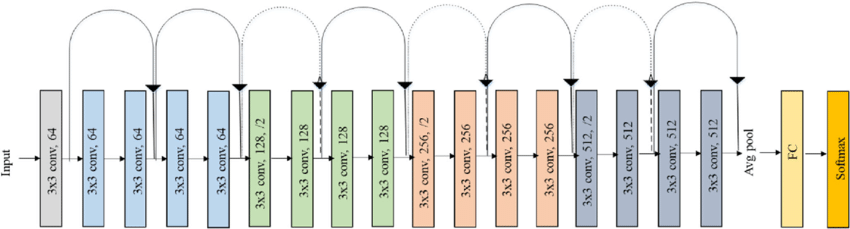
\includegraphics[width=1\textwidth]{ResNet18.png}
\caption{ResNet-18 Architecture}
\label{fig:resnet18}
\end{figure}

\subsubsection{Face recognition system implementation}

Before generating perturbation images from users’ photos, we need to build a facial recognition system to serve as the attacking target. Before we feed the facial images into ResNet, a critical step is to crop and extract the facial area from the input picture. To achieve this goal, we used MediaPipe to obtain the corner coordinates of the facial area.\\

Next, the cropped face area is fed to a ResNet-18 model. We applied transfer learning techniques to speed up the training process - we obtained the initial weight of the neural network from a pre-training task conducted on ImageNet. Then, we fine-tuned the ResNet model on our training set. Experimental results show that the fine-tuned model can effectively identify the facial identities in the test set. 


Here is a demonstration of our face-recognition system.

\begin{figure}[h]
    \centering
    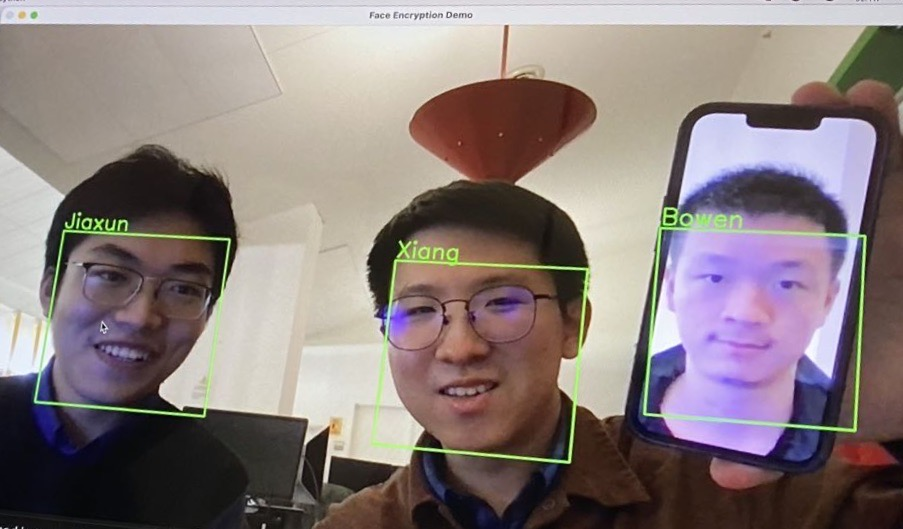
\includegraphics[width=0.6\textwidth]{face_recognition_demo.png}
    \caption{Face recognition system demo}
    \label{fig:face-recognition-demo}
    \end{figure}

\subsubsection{Performance}

\begin{figure}[h]
    \centering
    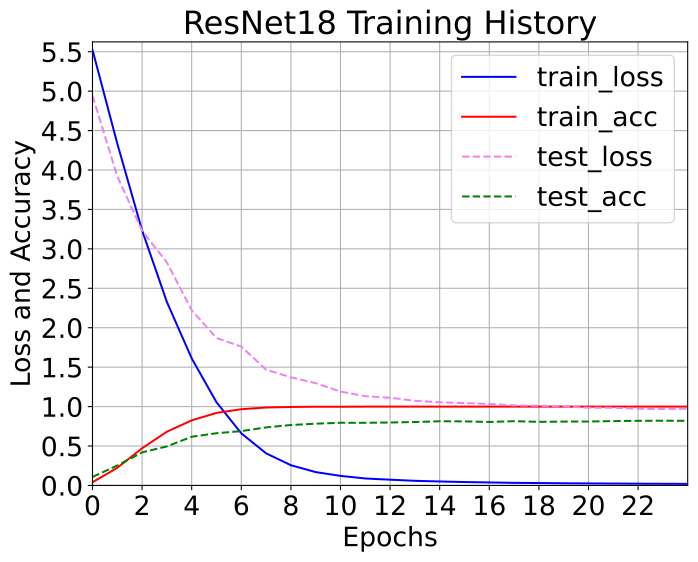
\includegraphics[width=0.5\textwidth]{Resnet18_performance.png}
    \caption{Resnet18 performance}
    \label{fig:resnet18_performance}
\end{figure}

Figure \ref{fig:resnet18_performance} demonstrates that with 25 epochs, the face recognition model Resnet-18 achieves 99.98\% accuracy on the training set and 81.93\% accuracy on the test set. We halted training at this point because any additional epoch would result in an overfitting problem.

\subsection{Adversarial Attacks}

% explain what is adversarial attacking

Adversarial attacking is a technique that can be used to fool machine learning models. It is a type of attack that aims to change the input data in a way that the model will misclassify it. The adversarial attacking technique is based on the fact that machine learning models are vulnerable to small perturbations in the input data. The perturbations are usually imperceptible to the human eye, but they can cause the model to misclassify the input data. \cite{adversarial_2020}

\begin{figure}[h]
    \centering
    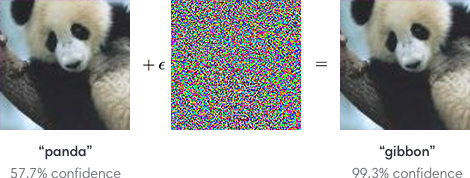
\includegraphics[width=0.8\textwidth]{adversarial_attack.png}
    \caption{An adversarial input, overlaid on a typical image, can cause a classifier to miscategorize a panda as a gibbon.}
    \label{fig:adversarial_attack}
\end{figure}

\subsubsection{PGD Attack}

The PGD attack is a white-box adversarial attack which means the attacker knows everything about the model, including gradients, model parameters and even the raining data and training procedure \cite{madry2017towards}. \\

In this project, we use the gradient of the loss function to generate adversarial examples. The attack is iterative and uses a step size to determine the size of the perturbation. The attack is also constrained by a maximum perturbation size.

\subsubsection{Non-Targeted Attack}

In a non-targeted attack, the goal is to generate an adversarial example that is misclassified by the target model $A$. Which means we are \textbf{maximizing} the loss function with respect to the target class $A$. The attack is as follows:\\

\begin{itemize}
    \item Input: \verb|face image|,\quad \verb|true label|,\quad \verb|face recognition model|
    \item Initialize: $\delta$ = random noise
    \item For each iteration: Modify the $\delta$ with step size according to gradient such that:\begin{center}
        \verb|Difference(Model(Face Image + Delta), True Label)| is maximum
    \end{center}

    \item Return $\delta$\\
\end{itemize}

where \verb|Model(Face Image + Delta)| is the prediction of perturbed data.

\subsubsection{Targeted Attack}

In a targeted attack, the goal is to generate an adversarial example that is misclassified $A$ by the target model and classified as a specific class $B$. Which means we are \textbf{minimizing} the loss function with respect to the target class $B$. The attack is as follows:\\

\begin{itemize}
    \item Input: \verb|face image|,\quad \verb|target label|,\quad \verb|face recognition model|
    \item Initialize: $\delta$ = random noise
    \item For each iteration: Modify the $\delta$ with step size according to gradient such that:\begin{center}
        \verb|Difference(Model(Face Image + Delta), Target Label)| is minimum
    \end{center}

    \item Return $\delta$\\
\end{itemize}

where \verb|Model(Face Image + Delta)| is the prediction of perturbed data.

\subsubsection{Real-Time Application}

Using the method described in the preceding section, we developed a program to execute PGD attacks through the camera in real time using the method described in the previous section. Before feeding them into the machine learning model, the application would capture images from the camera and then subject them to PGD perturbations. The output of the model would be monitored and the probability of the prediction would be displayed on the screen. This method allows for the testing and evaluation of machine learning models' resistance to PGD attacks in real time.


